\documentclass[a4paper]{jpconf}
\usepackage{graphicx}
\usepackage{mathtools}
\usepackage{amsmath}
\usepackage{multirow}
\usepackage{verbatim}
\usepackage[UKenglish]{babel}
\begin{document}
\title{Underwater Source Separation Using Multi-Stage Independent Component Analysis in Semi-Anechoic Water Tank}

\author{Ridhwan Juniarga Pribadi, Mifta Nur Farid, Wiratno Argo Asmoro, Wirawan, Endang Widjiati, Dhany Arifianto}

\address{Dept. of Engineering Physics, Faculty of Industrial Technology, Institut Teknologi Sepuluh Nopember, Kampus ITS Sukolilo, Surabaya 60111, Indonesia}

\ead{ridhwan.juniarga@gmail.com}

\begin{abstract}
The experiment of source separation in sea water environment often faced difficulties especially for controlling certain variables. One of the upcoming solution to simplify sea water environment was to conduct the experiment in the anechoic water tank. To evaluate the effects of the experiment performed in the water tank, the comparison of source separation using linear mixture and in-tank mixture will be analyzed. The source separation was performed in three different methods, Time Domain Independent Component Analysis (TDICA), Frequency Domain Independent Component Analysis (FDICA), and Multi Stage Independent Component Analysis (MSICA). The experiment result showing that compared to the linear mixture source, the performance of source separation degrade significantly while performed on the water tank, indicated by the MSE value which increased from $3^10^{-8}$ to $6^10^{-2}$. This result showing that the source mixture that occurred in water tank, much more complex compared to the linear mixture.
\end{abstract}

\section{Introduction}
Acoustic wave played important role in underwater communication.In terms of propagation and power attenuation, it performed better than electromagnetic wave in medium of water. However, the application of acoustic signals in ocean encountered many problems, such as limitation of bandwidth, huge noise environment, complexity of the medium itself, and the impact to surrounding marine biological life, thus required further processing in order to be used properly. Considering those level of complexity, a technique that is able to simplify the process of propagation modelling, as well as the reconstruction of the mixed sound was required.

References \cite{1} proposed one method of solving this problem by constructing a marine miniature in an anechoic water tank. By using this kind of tank as test-bed the fluctuation of important variables such as temperature, and salinity can be controlled and multipath channel can be eliminated.

By having proper experiment place, the modelling of propagation will be simplified, then Independent Component Analysis (ICA) will take place of sources separation. ICA is one of the method which estimate sources signal without any prior information about sources itself. One of the common method of ICA is Fast ICA, which in this paper will be called Time-Domain ICA (TDICA). The process of source mixing are formulated as common wave superposition (linear mixture). The drawback of this method came when facing signal which mixed in reverberant condition (convolutive mixture). In those condition, the propagation of source signal also impacted by the room impulse response, thus the assumption of independence and number of sources are less then sensors will collapse. Another method of ICA is to perform separation under frequency domain, which called Frequency Domain ICA (FDICA). This method will allow convolutive mixture to be simplify as linear mixture through Fourier Transform. However this methods also have drawback since the assumption of signal independence will collapse in each sub band. To overcome this problem, \cite{2} proposed to combine both of this methods in sequence, which called Multistage ICA (MSICA). In this method, signal estimation will be done in two stages, first in FDICA then followed by TDICA.

This paper will evaluated the quality of sources estimation using three of mentioned methods. The experiment conducted in water tank which belong to Vibration and Acoustic Laboratory, Institut Teknologi Sepuluh Nopember. The Performances of estimated signal will be evaluated in Mean Square Error (MSE) value by comparation to baseline signal. The MSE value of each method will be evaluated as function of distance of source and sensors.

\section{Determination of Test Signals}
There are two condition that have to be met by source signals. First, they have to be independent each other. It means that the first signal doesn’t contain any information of another signal. Second, the statistical distribution of the two sources signal are not gaussian distribution \cite{3}.

Using two preliminary requirement above, the signals below (Table \ref{table:source}) will be treated as the source signals of the experiment.

\begin{table}[h]
\centering
\caption{Source signal}
\label{table:source}
\begin{tabular}{|l|l|l|}
\hline
\multicolumn{1}{|c|}{No.} & \multicolumn{1}{c|}{Signal} & \multicolumn{1}{c|}{Note} \\ \hline
1.                        & Puretone 500 Hz             & Narrowband                \\ \hline
2.                        & Puretone 600 Hz             & Narrowband                \\ \hline
3.                        & Puretone 700 Hz             & Narrowband                \\ \hline
4.                        & Puretone 800 Hz             & Narrowband                \\ \hline
5.                        & Puretone 900 Hz             & Narrowband                \\ \hline
6.                        & Puretone 1 kHz              & Narrowband                \\ \hline
7.                        & Ship noise                  & Wideband stationary       \\ \hline
8.                        & Sonar pinging               & Wideband Non-stationary   \\ \hline
\end{tabular}
\end{table}

Each of the signal were recorded in 8000 Hz sampling frequency, 16 bit per sample, and have 4 seconds duration.

\section{Experiment Setup}
The Experiment was conducting in water tank which have dimension of 2 m length, 1 m width, and 1 m height. The Interior wall of tank was covered with absorber, to decrease the amount of reflection. The tank was filled with salt water which have salinity of 3.5\% and temperature of $25^o$C. The Velocity of sound in this condition is 1468.37 m/s.

\begin{figure}[h]
\begin{center}
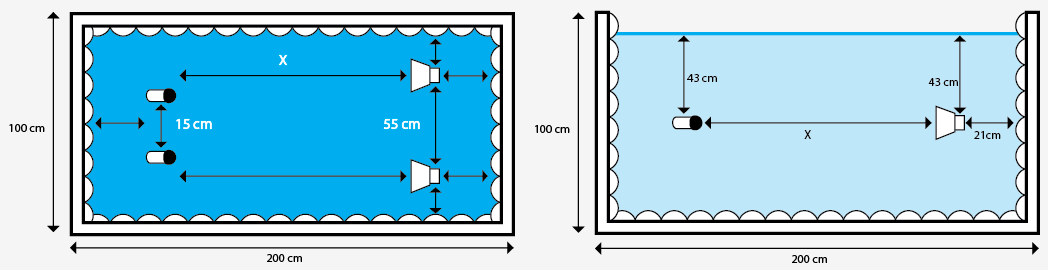
\includegraphics[width=5in]{experimentSetupwide.png}
\end{center}
\caption{\label{pict:setup}Experiment Setup. Side view (right) and top view (left)}
\end{figure}

The configuration of sources and sensor can be seen in Figure \ref{pict:setup}. There are three variations of the distance between the hydrophone-speakers are 85 cm, 1 m, and 1.5 m. The number of sensors is two, so does the sources. The distance of each sensor is 15 cm, while the distance of each speaker is 55 cm.

\section{Time Domain Independent Component Analysis (TDICA)}
In the case of linear mixture, mixed signal is just sum or superposition of each source followed by some gain. This assumption can be formulated as $X(t)=A \cdot S(t)$, where $X(t)$ is vector matrix of mixed signal, $S(t)$ is vector matrix of source signal, and $A$ is mixing matrix of signal. Using above equation, then the source can be estimated by finding the inverse of $A$.

Since ICA using iteration process to estimate inverse of A, which quite time consuming if it is applied in real time world, there exist some preprocessing method in order to shorten the iteration process. First step is centering the signal. This step intended to make zero-mean signal observation using equation, $X_c(t) = X(t) - E(X)$, where $X_c(t)$ is centered vector signal, and $E(X)$ is the signal expectation.

After signal have been centered, it will be get to whitening process. This step intend to make recorded signal uncorrelated each other by using Eigenvalue Decomposition, $V = \frac{E}{\sqrt{D}}E^T$. Where $V$ is whitening matrix, $E$ is orthogonal matrix of eigenvector of $E(XX^T)$, and $D$ is diagonal matrix of its eigenvalues. After $V$ acquired, whitened signal can be obtained by using equation, $X_w(t) = V X_c(t)$

After signal being preprocessed, the estimation of source signal will be accomplished using ICA algorithm. In this experiment, algorithm of \cite{5} was applied to estimate source signal. The principle of this algorithm was to minimize the entropy of estimated signal, since the low entropy is one of the feature of independence signal, and high entropy is the characteristic of gaussian random variable.

\begin{equation}\label{pers:entropy}
L = \sum_{t=1}^T \sum_{i=1}^n log f_i \left(w_i^T x(t)\right) ~+~ T log |det W|
\end{equation}

Demixing matrix is optimized using this epoch, $W^+ = W + \mu\left[I + f(X)X^T\right]W$, where $g(y)$ is non linear function, in this paper $Tanh(y)$ was used. Then the estimation signal acquired by using equation, $Y(t) = WX_w(t)$.

After estmation source $Y(t)$ acquired, it will be compared to the baseline signal to evaluate the quality of source separation using equation (\ref{pers:mse}).

\begin{equation}\label{pers:mse}
MSE = \frac{1}{M} \sum_{m-1}^M \left(s[m] - y[m]\right)^2
\end{equation}

Figure \ref{pict:msetdica} shows the score of estimated signal using TDICA. Lower value of MSE indicated better separation performance.

\begin{figure}[h]
\begin{center}
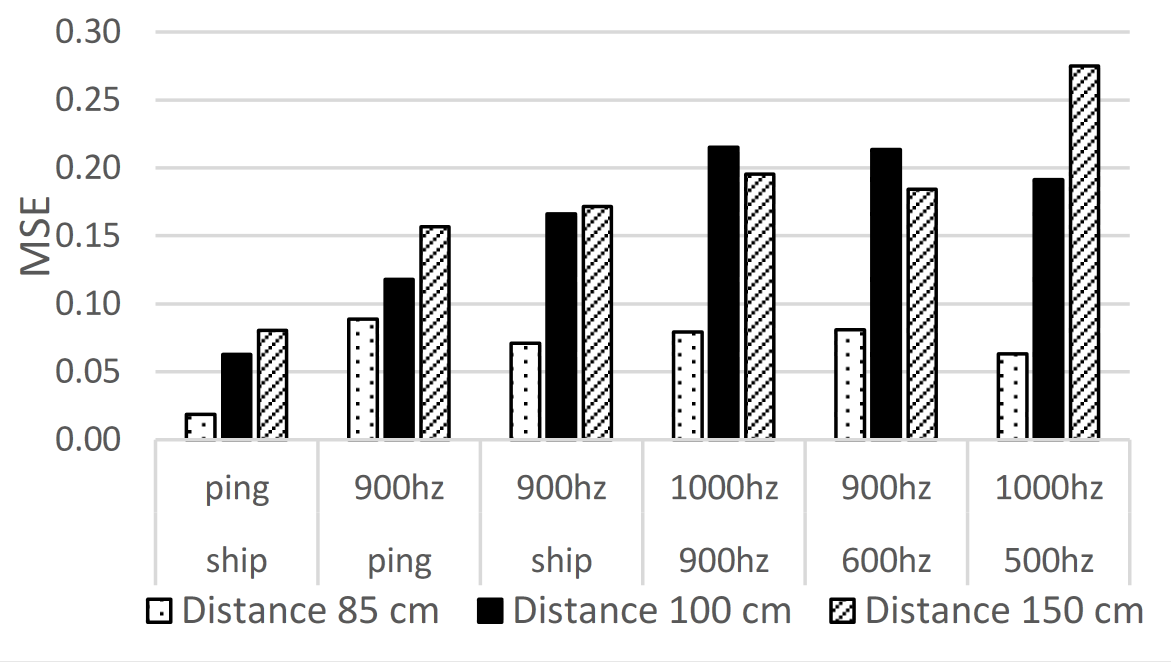
\includegraphics[width=3in]{figure2.png}
\caption{\label{pict:msetdica}Result of mixed signal separation using TDICA indicated by its MSE.}
\end{center}
\end{figure}

\section{Frequency Domain Independent Component Analysis (FDICA)}
If the mixing process is not just simple superposition of each sources, in other word the signal recording performed in reverberant condition, convolutive mixture model have to be taken. This model accommodate room impulse response as the Finite Impulse Response (FIR) filter of mixed signal.

It is shown in equation, $X(t) = \sum_{n=0}^{N-1}A^{(t)}(n)S(t-n)$, where $N$ is the length of FIR filter. If the length of reverberation is 0.5 s and our recording frequency sampling is 8000 Hz, the length of FIR is 4000 taps, thus the number of demixing matrix W(n) that need to be estimated is just same in number. In order to simplify the calculation process, \cite{6} proposed to tansforming this equation in frequency domain, $X(f)=A(f)S(f)$.

In this paper, this is achieved by performing ICA after signal being transformed in frequency domain using Fast Fourier Transform (FFT) algorithm. After demixing matrix estimated so does the signal estimation in frequency domain, it will be transformed back to time domain using Inverse Fast Fourier Transform (IFFT), then the quality of estimation signal will be acquired by comparing to baseline signal. The MSE value of each FDICA estimation signal are shown in Table \ref{pict:msefdica}.

\begin{figure}[h]
\begin{center}
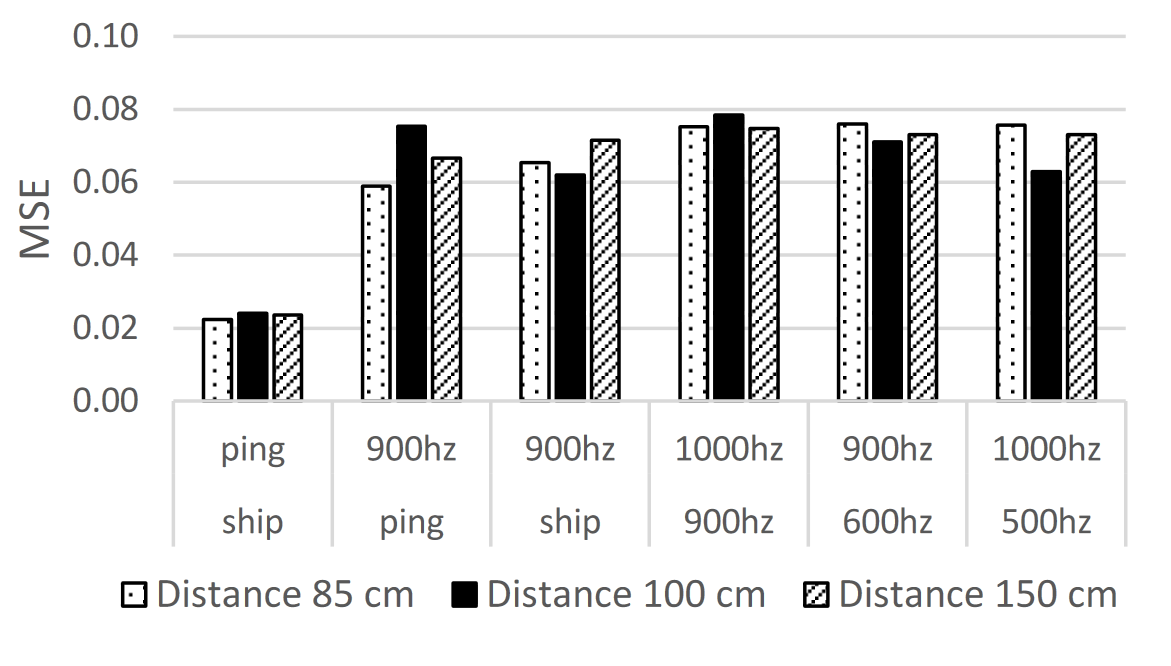
\includegraphics[width=3in]{figure3.png}
\caption{\label{pict:msefdica}Result of mixed signal separation using FDICA indicated by its MSE.}
\end{center}
\end{figure}

\section{Multistage Independent Component Analysis (MSICA)}
Although FDICA can resolve the complexity of convolutive mixture, it also have some disadvantage. When the signal being transformed into frequency domain, it lost the independence assumption (since the independence assumption is statistical feature that exist in time domain), thus the separation performance will be saturated before reaching sufficient performance. 

In order to resolve this problem, \cite{2} proposed new algorithm to combine FDICA and TDICA which called MSICA. In this method, FDICA and TDICA are performed sequentially. FDICA was performed in the first stage, then estimated signal of FDICA will be feed as the input of second stage TDICA. The MSE value of each MSICA estimation signal are shown in Table \ref{pict:msemsica}.

\begin{figure}[h]
\begin{center}
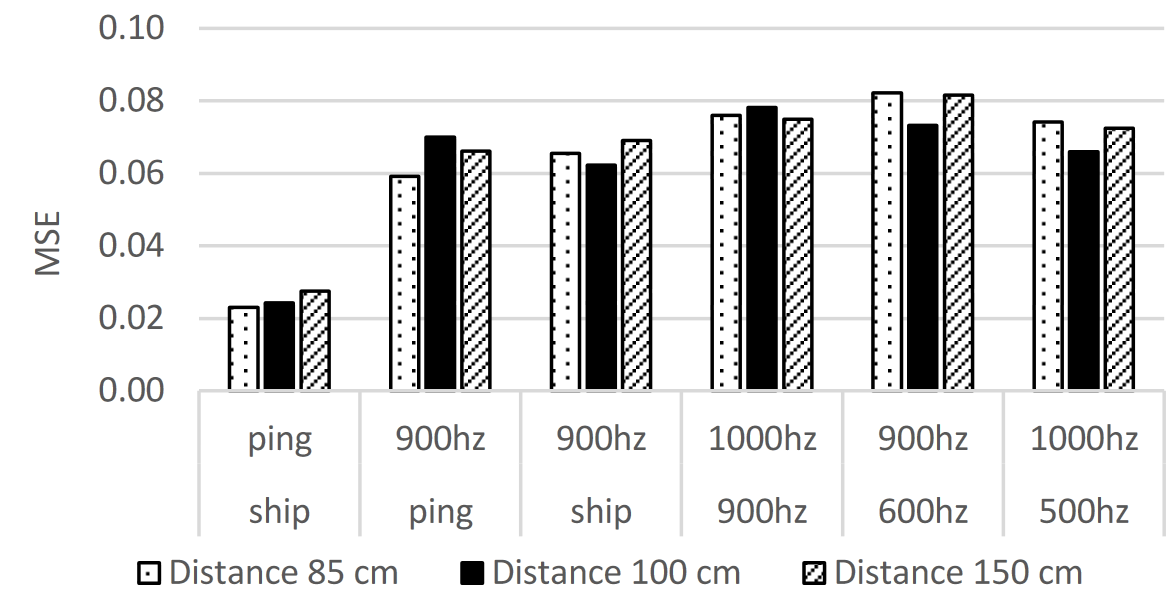
\includegraphics[width=3in]{figure5.png}
\caption{\label{pict:msemsica}Result of mixed signal separation using MSICA indicated by its MSE.}
\end{center}
\end{figure}
\section{Discussion}
Comparison of the performance of each method can be seen in Figure \ref{pict:comparison}. Total MSE of of each signal estimation is averaged to obtain the MSE of each method.

\begin{figure}[h]
\begin{center}
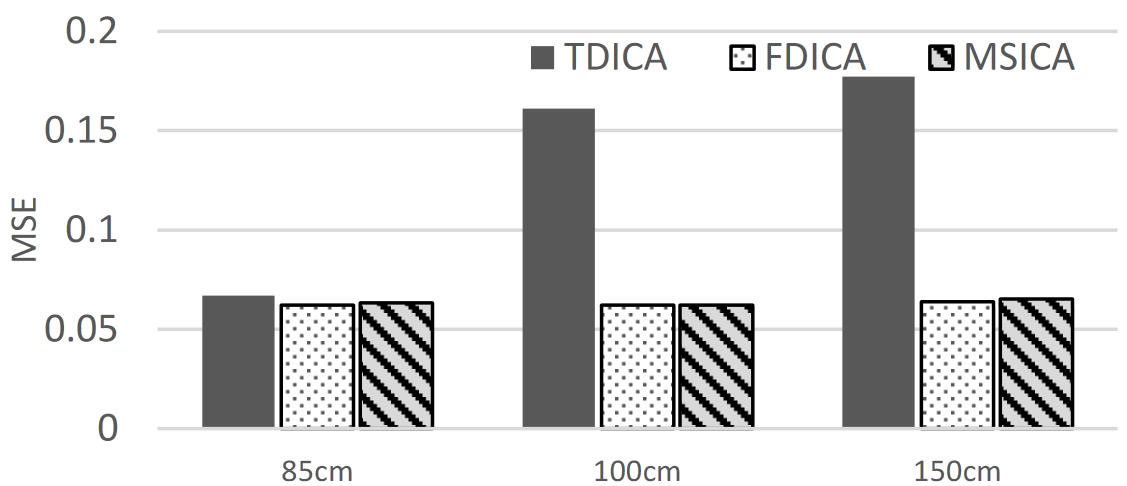
\includegraphics[width=3in]{figure6.png}
\caption{\label{pict:comparison}Comparison of the average value of the MSE Each separation method. MSICA and FDICA has identical score. In contrast, the performance of the method TDICA decreases as the increasing of distance between sources and sensors}
\end{center}
\end{figure}

In the distance of 85cm, TDICA, FDICA, and MSICA have similar performances, but eventually as the distance increase, performance of TDICA was decrease. FDICA and MSICA gave stable result of MSE value. There are two explanation of this event. First, the performance of source separation decrease as the intensity of signal get attenuated by propagation, in other words the SNR of signal play big role. Second, as the distance increase, the ratio of indirect sound to direct sound got bigger due to the scattering. Since the FDICA and MSICA shown stable performances, as shown in Figure \ref{pict:comparison}, the first assumption got weak, and second assumption is more dependable. 

The reason of this hypothesis was the changing of signal distribution in the addition of distance as shown in Figure \ref{pict:gausDist}. It is show that the distribution of both signal tends to be Gaussian for the increasing of distance. According to the central limit theorem, the distribution of independent component summation, tends to be Gaussian distribution, hence the assumption of instantaneous mixture collapsed.

In underwater communication the scattering occurred when the sound wave faces different temperature and salinity due to the increasing water pressure by depth of water. Since the tank had homogen salinity and temperature, the scattering suspected came from the surface of the water. The surface of the water act as a boundary between two different medium, which is water and air. This two different medium has different characteristic of sound propagation. This made the sound wave that came to the surface will be scattered. Another suspect of scattering is due to reflection of the wall. Since the wall have been covered by the absorber, the indirect sound wave that came from this event won’t be bigger than from the surface. 

\begin{figure}[h]
\begin{center}
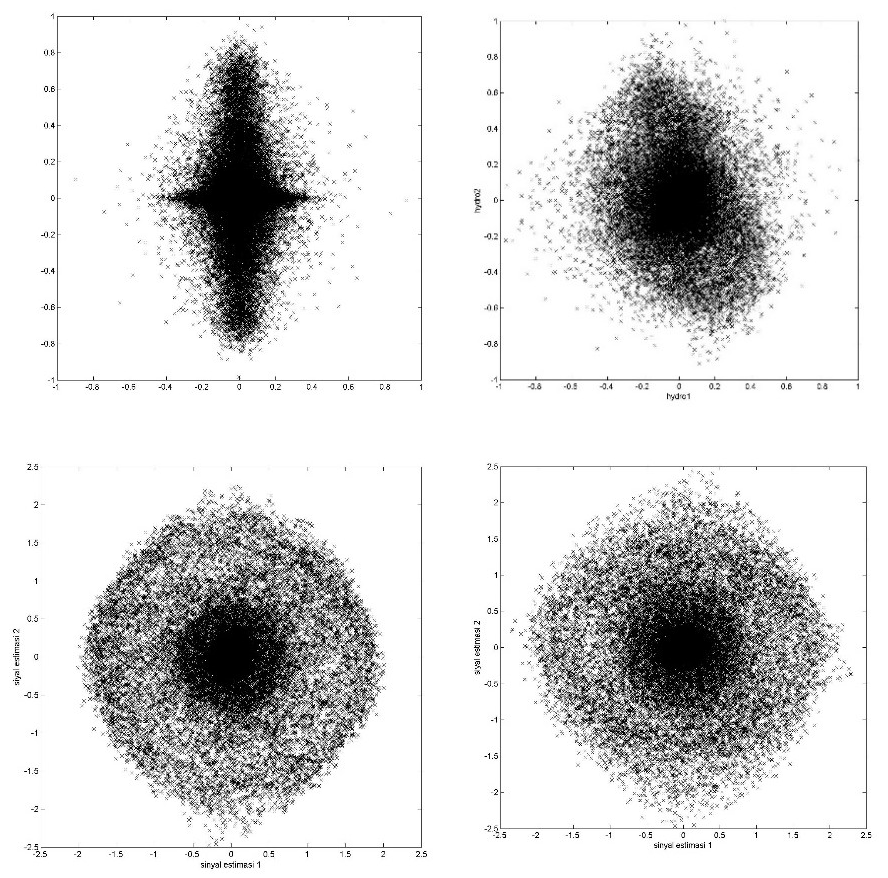
\includegraphics[width=3in]{gausDist.png}
\caption{\label{pict:gausDist}Distribution of Testing Signal Ship dan Ping; baseline (top-left); distance 85 cm (top-right); distance 100 cm (bottom-left); distance 150 cm(bottom-right).}
\end{center}
\end{figure}

\section{Conclusion}
\renewcommand{\theenumi}{\arabic{enumi}}
\begin{enumerate}
\item Pre-filtering is required in data acquistision stage to eliminate the effect of harmonic distortion generated by the speaker.
\item The water tank impulse response can be accounted while modelling the convolutive mixture, in order to get better simmulation.
\item Additional measurement position in variation of depth need to be add in order to have understanding major source of scattering.
\end{enumerate}

\section*{References}
\begin{thebibliography}{9}
\bibitem{1} Cochard, N., Lacoume, J. L. 2000 “Underwater Acoustic Noise Measurement in Test Tank”.IEEE Journal of Oceanic Engineering, 25(1).
\bibitem{2} Nishikawa, T., Saruwatari, H., dan Shikano, K. 2003. "Blind Source Separation of Acoustic Signals Based on Multistage ICA Combining Frequency-Domain ICA and Time-Domain ICA". IEICE Trans. Fundamentals, E86-A (4)
\bibitem{3} Hyvarinen, A., Karhunen, J., dan Oja, E. 2001, "Independent Component Analysis: Basic Independent Component Analysis".NewYork: John Willey \& Sons.
\bibitem{5} Bell, Sejnowski, 1995. ” An Information-Maximization Approach to Blind Separation and Blind Deconvolution”, Neural computation, vol. 7, no. 6, pp. 1129–1159.
\bibitem{6} Kawamoto, M., Matsuoka, K., dan Ohnishi, N. 1998. "A method of blind separation for convolved non-stationary signals". Elsevier Neurocomputing 22 :157-171
\end{thebibliography}
\end{document}